\documentclass[man]{apa6}
\usepackage{lmodern}
\usepackage{amssymb,amsmath}
\usepackage{ifxetex,ifluatex}
\usepackage{fixltx2e} % provides \textsubscript
\ifnum 0\ifxetex 1\fi\ifluatex 1\fi=0 % if pdftex
  \usepackage[T1]{fontenc}
  \usepackage[utf8]{inputenc}
\else % if luatex or xelatex
  \ifxetex
    \usepackage{mathspec}
  \else
    \usepackage{fontspec}
  \fi
  \defaultfontfeatures{Ligatures=TeX,Scale=MatchLowercase}
\fi
% use upquote if available, for straight quotes in verbatim environments
\IfFileExists{upquote.sty}{\usepackage{upquote}}{}
% use microtype if available
\IfFileExists{microtype.sty}{%
\usepackage{microtype}
\UseMicrotypeSet[protrusion]{basicmath} % disable protrusion for tt fonts
}{}
\usepackage{hyperref}
\hypersetup{unicode=true,
            pdftitle={Reproducing the Mehr, Song \& Spelke (2016)},
            pdfauthor={Zoren Degtyarev~\& Ernst-August Doelle},
            pdfkeywords={music, social cognition, memory, infant development, open data, open
materials},
            pdfborder={0 0 0},
            breaklinks=true}
\urlstyle{same}  % don't use monospace font for urls
\usepackage{graphicx,grffile}
\makeatletter
\def\maxwidth{\ifdim\Gin@nat@width>\linewidth\linewidth\else\Gin@nat@width\fi}
\def\maxheight{\ifdim\Gin@nat@height>\textheight\textheight\else\Gin@nat@height\fi}
\makeatother
% Scale images if necessary, so that they will not overflow the page
% margins by default, and it is still possible to overwrite the defaults
% using explicit options in \includegraphics[width, height, ...]{}
\setkeys{Gin}{width=\maxwidth,height=\maxheight,keepaspectratio}
\IfFileExists{parskip.sty}{%
\usepackage{parskip}
}{% else
\setlength{\parindent}{0pt}
\setlength{\parskip}{6pt plus 2pt minus 1pt}
}
\setlength{\emergencystretch}{3em}  % prevent overfull lines
\providecommand{\tightlist}{%
  \setlength{\itemsep}{0pt}\setlength{\parskip}{0pt}}
\setcounter{secnumdepth}{0}
% Redefines (sub)paragraphs to behave more like sections
\ifx\paragraph\undefined\else
\let\oldparagraph\paragraph
\renewcommand{\paragraph}[1]{\oldparagraph{#1}\mbox{}}
\fi
\ifx\subparagraph\undefined\else
\let\oldsubparagraph\subparagraph
\renewcommand{\subparagraph}[1]{\oldsubparagraph{#1}\mbox{}}
\fi

%%% Use protect on footnotes to avoid problems with footnotes in titles
\let\rmarkdownfootnote\footnote%
\def\footnote{\protect\rmarkdownfootnote}


  \title{Reproducing the Mehr, Song \& Spelke (2016)}
    \author{Zoren Degtyarev\textsuperscript{1}~\& Ernst-August
Doelle\textsuperscript{1,2}}
    \date{}
  
\shorttitle{For Infants Melodies Are Social}
\affiliation{
\vspace{0.5cm}
\textsuperscript{1} Brooklyn College of the City University of New York\\\textsuperscript{2} Konstanz Business School}
\keywords{music, social cognition, memory, infant development, open data, open materials\newline\indent Word count: X}
\usepackage{csquotes}
\usepackage{upgreek}
\captionsetup{font=singlespacing,justification=justified}

\usepackage{longtable}
\usepackage{lscape}
\usepackage{multirow}
\usepackage{tabularx}
\usepackage[flushleft]{threeparttable}
\usepackage{threeparttablex}

\newenvironment{lltable}{\begin{landscape}\begin{center}\begin{ThreePartTable}}{\end{ThreePartTable}\end{center}\end{landscape}}

\makeatletter
\newcommand\LastLTentrywidth{1em}
\newlength\longtablewidth
\setlength{\longtablewidth}{1in}
\newcommand{\getlongtablewidth}{\begingroup \ifcsname LT@\roman{LT@tables}\endcsname \global\longtablewidth=0pt \renewcommand{\LT@entry}[2]{\global\advance\longtablewidth by ##2\relax\gdef\LastLTentrywidth{##2}}\@nameuse{LT@\roman{LT@tables}} \fi \endgroup}


\DeclareDelayedFloatFlavor{ThreePartTable}{table}
\DeclareDelayedFloatFlavor{lltable}{table}
\DeclareDelayedFloatFlavor*{longtable}{table}
\makeatletter
\renewcommand{\efloat@iwrite}[1]{\immediate\expandafter\protected@write\csname efloat@post#1\endcsname{}}
\makeatother
\usepackage{lineno}

\linenumbers

\authornote{Add complete departmental affiliations for each
author here. Each new line herein must be indented, like this line.

Enter author note here.

Correspondence concerning this article should be addressed to Zoren
Degtyarev, Postal address. E-mail:
\href{mailto:zoren@gmail.com}{\nolinkurl{zoren@gmail.com}}}

\abstract{
A reproduction of the analysis for Experiment 1 from Mehr, Song \&
Spelke (2016). Five month old infants were exposed to one of two novel
songs containing different melodies with lyrics and rhythms being the
same. Infants either heard the songs through a toy in which their
parent's voice was recorded or heard it live by a friendly unfamiliar
person initially and later through video recording. Infant's selective
attention was tested by having them listen to two presentations of
either familiar or unfamiliar songs. Infants payed attention to the
familiar song, sung by their parent in the past. No infant preference
was observed between the toy onto which parent's voice was recorde or a
video recording of an unfamiliar person, briefly met by an infant
initially. Infants in the later two conditions retained the memory of
the melody for longer than 8 months. These findings suggest that songs
performed by parents at home convey social meaning to a child.


}

\begin{document}
\maketitle

This is an example of creating an APA manuscript using papaja, and also
an example for part 2 (APA paper in R markdown) of the midterm
assignment. This script will enable to recreate APA style manuscripts
using R markdown. This report re-produces the analysis of Experiment 1
reported in Mehr, Song \& Spelke (2016) ({\textbf{???}}). The data were
downloaded from
\url{https://github.com/693284/papajaTest/blob/master/MehrSongSpelke2016.csv}
Music is universal to most human beings. Children and infants often
listen to their parents' singing. Parents usually sing in a style
relatable across different cultures. What is the reason behind children
paying attention to these types of songs? Mehr and his colleagues in
2016 tested the hypothesis that melodies convey social meaning to
infants. Specifically, these melodies inform us about social bonding.
Mehr and colleugues assert that children are exposed to melodies that
are shared within a specific social group. As children grow up in a
specific culture, childrent get exposed to certain tune or songs (e.g.,
\enquote{Babushka Baio}), while in a different culture a child might be
exposed to a different song (e.g., \enquote{My Little Love}). Thus, when
an infant hears a stranger singing a song that a child recognizes, this
song may convey crucial information that this stranger can belong to the
same social group. To test whether this is so, the researchers conducted
an experiment in which they recruited 32 infants with their parents. The
experiment had two phases. During the first phase the participants
visited to the lab during which the parents were taught a new lullaby
that neither the parents nor thier child heard prior. After learning the
new lullaby, parents sang it to their child every day for the next 1-2
weeks. After the completion of the exposure period, participants (parent
and thier infant) returned to the lab to complete the second phase of
the experiment in which infants first saw a screen with side-by-side
videos of two strangers. Strangers were silently smiling while looking
at the infant. To establish a baseline, infant's gaze direction was
recorded. Following the baseline recordings, infants saw two strangers
on the screen, singing either the lullaby that the perents learned in
the first phase of the experiment or a different lullaby containing
different melody but with the same lyrics and rhythm. Please refer to
Mehr et al. (2016) Experiment 1 for more details on experiment's
methods.

\section{Methods}\label{methods}

We report how we determined our sample size, all data exclusions (if
any), all manipulations, and all measures in the study.

\subsection{Participants}\label{participants}

There were 32 participants (5 month old infants; 17 females; mean age =
5.61 months, SD = 0.31, range: 5.06--6.11)

\subsection{Material}\label{material}

The details of the Melodies are Social for Infants experiment are
reported in Mehr et.al, (2016)

\subsection{Procedure}\label{procedure}

The infant sat on his or her parent's lap, about 5 ft away from a 55- ×
40-in. projection screen. During the experiment the parent had to sit
with his or her eyes closed as well as had to wear noise-canceling
headphones that played masking music. Testing the selective-attention
included four parts. Infant first saw side-by-side high-definition video
recordings of the two strangers, smiling while directly looking at the
infant, for 16 s (baseline trial). Next, the infant saw, first, one 22-s
video of each of the two strangers singing one of the two songs while
keep looking and smiling at the infant (familiarization trials).
Finally, the infant watched a silent 16-s test trial that was precise to
the baseline trial. To keep infant's eyes attending to the center of the
screen before the baseline and test trials, researchers made an object
with an attractive sound appear at the center of the screen. \#\# Data
analysis We used R (Version 3.5.2; R Core Team, 2018) and the R-packages
\emph{data.table} (Version 1.12.0; Dowle \& Srinivasan, 2019),
\emph{dplyr} (Version 0.8.0.1; Wickham, François, Henry, \& Müller,
2019), \emph{papaja} (Version 0.1.0.9842; Aust \& Barth, 2018),
\emph{pwr} (Version 1.2.2; Champely, 2018), and \emph{summarytools}
(Version 0.9.2; Comtois, 2019) for all our analyses.

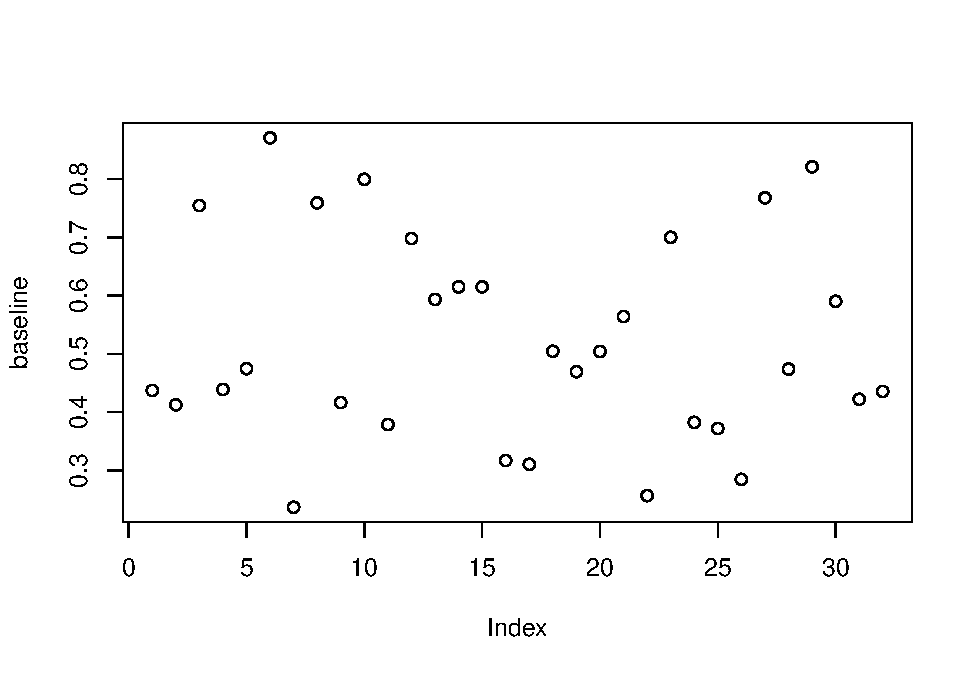
\includegraphics{Midterm_files/figure-latex/unnamed-chunk-5-1.pdf} \#
Results

\begin{verbatim}
## [1] 0.5210967
\end{verbatim}

\begin{verbatim}
## [1] 0.1769651
\end{verbatim}

Mean proportion of time that infants looked at two strangers shows to be
closer to 50/50

\begin{verbatim}
## 
##  One Sample t-test
## 
## data:  baseline
## t = 0.67438, df = 31, p-value = 0.5051
## alternative hypothesis: true mean is not equal to 0.5
## 95 percent confidence interval:
##  0.4572940 0.5848994
## sample estimates:
## mean of x 
## 0.5210967
\end{verbatim}

The mean proportion looking time toward the singing stranger during
Experiment 1 was .52, and was not significantly different from .5 (50/50
chance), according to a one-sample test, t(31) = .67, p = .505.

\section{Discussion}\label{discussion}

The re-analysis successfully reproduced the analysis reported by Mehr et
al. (2016) In the following section, I show an example of completing a
simulation based power analysis for this design.

\subsection{Simulation-based power
analysis}\label{simulation-based-power-analysis}

\newpage

\section{References}\label{references}

\begingroup
\setlength{\parindent}{-0.5in} \setlength{\leftskip}{0.5in}

\hypertarget{refs}{}
\hypertarget{ref-R-papaja}{}
Aust, F., \& Barth, M. (2018). \emph{papaja: Create APA manuscripts with
R Markdown}. Retrieved from \url{https://github.com/crsh/papaja}

\hypertarget{ref-R-pwr}{}
Champely, S. (2018). \emph{Pwr: Basic functions for power analysis}.
Retrieved from \url{https://CRAN.R-project.org/package=pwr}

\hypertarget{ref-R-summarytools}{}
Comtois, D. (2019). \emph{Summarytools: Tools to quickly and neatly
summarize data}. Retrieved from
\url{https://CRAN.R-project.org/package=summarytools}

\hypertarget{ref-R-data.table}{}
Dowle, M., \& Srinivasan, A. (2019). \emph{Data.table: Extension of
`data.frame`}. Retrieved from
\url{https://CRAN.R-project.org/package=data.table}

\hypertarget{ref-R-base}{}
R Core Team. (2018). \emph{R: A language and environment for statistical
computing}. Vienna, Austria: R Foundation for Statistical Computing.
Retrieved from \url{https://www.R-project.org/}

\hypertarget{ref-R-dplyr}{}
Wickham, H., François, R., Henry, L., \& Müller, K. (2019). \emph{Dplyr:
A grammar of data manipulation}. Retrieved from
\url{https://CRAN.R-project.org/package=dplyr}

\endgroup


\end{document}
